\chapter{Convertidores A/D}
% La variedad de circuitos empleados para la conversión A/D es mayor que en convertidores D/A.

\section{Convertidores A/D paralelos}

Los denominados convertidores <<flash>> son un tipo de CAD paralelo que consisten, para $n$ bits, en un divisor de tensión con $2^{n-1}$ tomas intermedias. Cada toma se conecta a un comparador analógico de alta velocidad, cuya otra entrada va conectada a la tensión a convertir. Este método de conversión es el más rápido disponible comercialmente. Su principal inconveniente es que necesita $2^{n-1}$ comparadores, por lo que sólo puede concebirse como CI LSI, no a base de componentes discretos.

\begin{figure}[H]
    \centering
    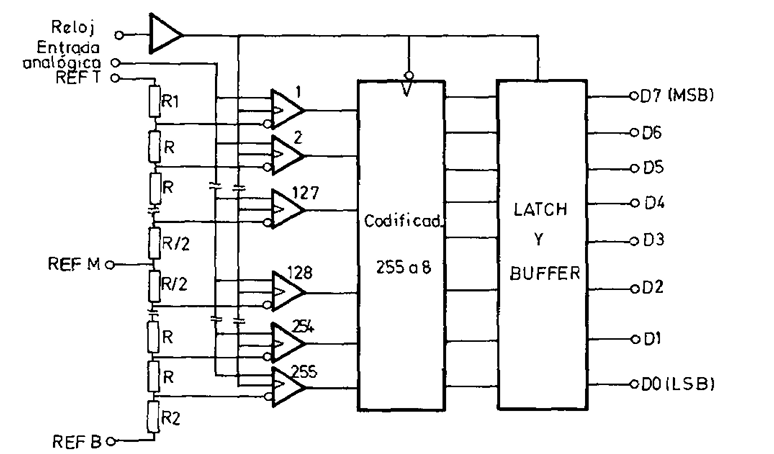
\includegraphics[width=0.75\linewidth]{Imagenes/Convertidor AD paralelo.png}
    \caption{Diagrama de bloques del convertidor paralelo TLC5502 (\textit{Texas Instruments})}
\end{figure}

\section{Convertidores de aproximaciones sucesivas}

El algoritmo de aproximaciones sucesivas ofrece un buen compromiso entre velocidad y complejidad, y es el más frecuente cuando no se trata de obtener una exactitud muy elevada. Hay muchos modelos de 8, 10, 12, 14 y 16 bits, con tiempos de conversión entre 1 y 100$\mu$s. Se puede montar con componentes discretos, pero su coste supera el de muchos de los CI disponibles.

El método consiste en ir comparando la tensión de entrada con una tensión analógica generada internamente con un CDA, cuya entrada digital incrementa o decrementa según que el resultado de la comparación indique, respectivamente, que la tensión de entrada es inferior o superior a la tensión generada internamente. Los errores del CDA pueden llevar a no linealidades.

El tiempo de conversión aumenta al hacerlo la resolución deseada, pero es independiente de la amplitud de la entrada. El límite actual es de unas $10^6$ conversiones para 12 bits. Dado que el resultado de una comparación no se fija en el registro de salida hasta que llega el ciclo del reloj siguiente a aquel en el que se ha efectuado la comparación, si la frecuencia de reloj es $f_r$ el tiempo de conversión para $n$ bits es:

\begin{equation}
    t_c = \frac{n + 1}{f_r}
\end{equation}

Un inconveniente de este método es su no linealidad si la entrada varía durante el tiempo de conversión. Para evitar que la entrada cambie durante la conversión, se precede al CAD con un amplificador S\&H; esto no evita, sin embargo, que la muestra tomada pueda venir influida por el posible ruido en la entrada. En cualquier caso son, pues, convertidores muy susceptibles al ruido.

\begin{figure}[H]
     \centering
     \begin{subfigure}[b]{0.45\textwidth}
         \centering
         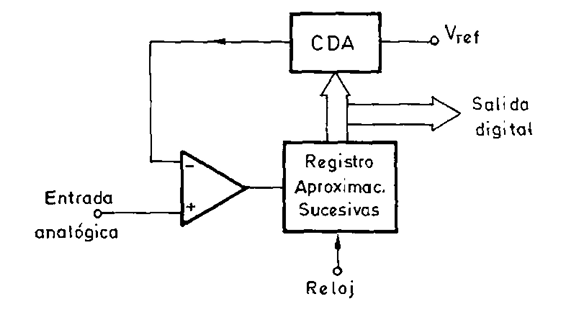
\includegraphics[width=\textwidth]{Imagenes/Convertidor de aproximaciones sucesivas.png}
         \caption{Esquema simplificado de un CAD basado en el algoritmo de aproximaciones sucesivas.}
     \end{subfigure}
     \hfill
     \begin{subfigure}[b]{0.45\textwidth}
         \centering
         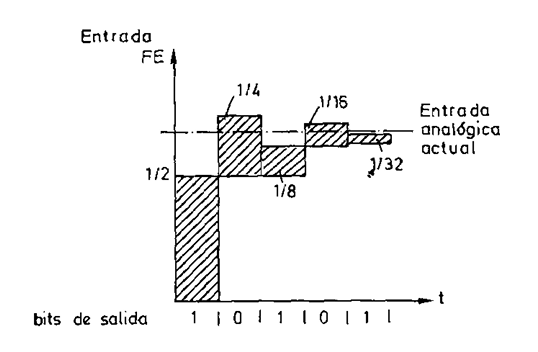
\includegraphics[width=\textwidth]{Imagenes/Convertidor Aproximaciones Sucesivas Bits.png}
         \caption{Asignación de valor a los bits de salida en comparaciones sucesivas.}
     \end{subfigure}
    \caption{}
\end{figure}

\section{Convertidores tipo servo}

Este tipo de convertidor está basado también en la comparación de la entrada con una tensión analógica generada con un CDA, pero en este caso la palabra digital es la salida de un contador bidireccional. Al iniciar la conversión, el contador se pone a cero, y su salida va incrementando hasta que rebasa el valor de la entrada, situación que es detectada por el comparador. Una vez ha <<alcanzado>> a la entrada, cualquier posible cambio pequeño en ésta es seguido rápidamente, contando o descontando, y de ahí la analogía como un servosistema.

La máxima velocidad (SR, \textit{Slew Rate}) de la señal de entrada que el sistema realimentado puede seguir, está limitada por la frecuencia de reloj $f_r$.

\begin{figure}[H]
    \centering
    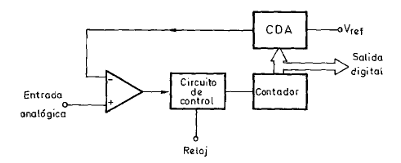
\includegraphics[width=0.75\linewidth]{Imagenes/Convertidores tipo servo.png}
    \caption{Convertidor A/D tipo servo \textit{tracking}.}
\end{figure}

\section{Convertidores sigma-delta}

Conocidos también como convertidores delta-sigma, convertidores de 1 bit y convertidores con sobremuestreo, se están convirtiendo en los favoritos para aplicaciones de alta resolución a frecuencias bajas y medias. Constan de un modulador analógico y de un circuito de filtrado y diezmado. El modulador analógico convierte la señal de entrada en una salida de dos niveles (1 bit) y alta velocidad (de aquí el <<sobremuestreo>>), y consta de uno o varios integradores, un comparador cuya salida se almacena en un cerrojo, y un CDA de 1 bit (o más en algunos modelos). El circuito sustrae (de ahí la <<delta>>) la salida del CDA de la entrada analógica e integra (de ahí la <<sigma>>) el resultado. La salida del integrador se compara con cero a alta velocidad, de modo que se tiene una secuencia de unos y ceros a alta velocidad. El CDA en el lazo de realimentación intenta mantener la salida del integrador próxima a cero; puede ser una simple fuente de corriente. El filtro digital elimina el ruido de alta frecuencia introducido por el modulador analógico. El diezmador ofrece las muestras de salida a una velocidad menor de la disponible a la salida del comparador, pero con mayor resolución.

\begin{figure}[H]
    \centering
    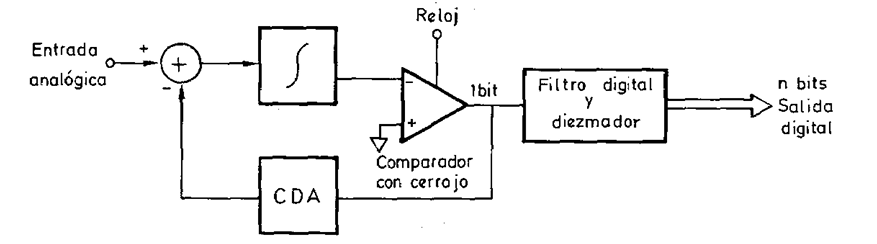
\includegraphics[width=0.75\linewidth]{Imagenes/Convertidores sigma delta.png}
    \caption{Estructura básica de un CAD sigma-delta.}
\end{figure}

\section{Convertidores de rampa: simple y doble}
Este método de conversión consiste en convertir primero la tensión de entrada en otra magnitud, y después convertir esta magnitud en una salida digital. En los denominados convertidores de rampa, la magnitud intermedia es el intervalo de tiempo de carga o descarga de un condensador.

En el caso de rampa simple, se integra la tensión de referencia hasta que la salida del integrador iguala a la tensión de entrada. El tiempo que se tarda en llegar a esta situación depende de la magnitud de la tensión de entrada, y se mide con un reloj y un contador internos. La precisión depende de la frecuencia del reloj, de la estabilidad de la tensión de referencia y de la capacidad del condensador de integración.

\begin{figure}[H]
    \centering
    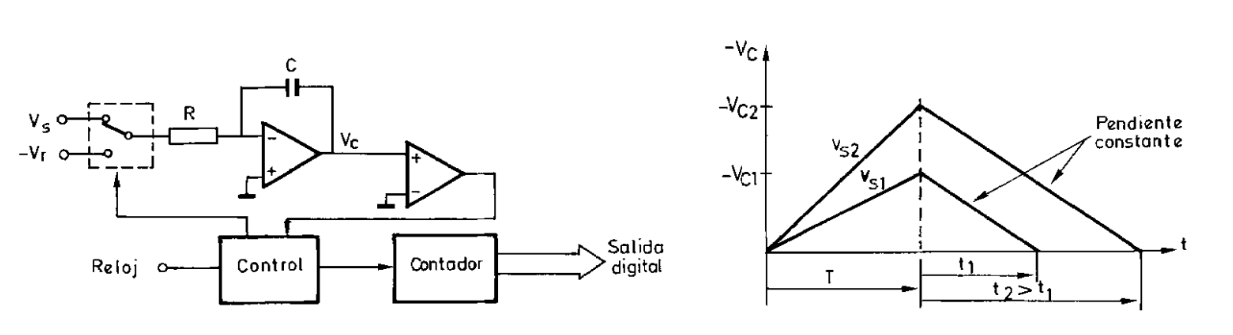
\includegraphics[width=0.75\linewidth]{Imagenes/Convertidor Doble Rampa.png}
    \caption{Convertidor A/D de doble rampa.}
\end{figure}

En los convertidores de doble rampa, se integra la señal de entrada $v_s$, constante, en un condensador durante un tiempo prefijado $T$, y luego se descarga el condensador hasta cero, empleando una corriente conocida determinada por la tensión de referencia, $V_r$. En la fase de integración, la tensión en el condensador alcanza un valor

\begin{equation}
    V_C = \frac{1}{\tau} \int_{0}^{T} - v_s dt = \frac{v_s}{\tau}T
\end{equation}

donde $\tau = R C$ es la constante de tiempo del integrador. La descarga hasta $0 V$, empleando la tensión de referencia $-V_r$, para establecer la corriente de descarga, dura un tiempo $t$ tal que

\begin{equation}
    0 - v_s = \frac{1}{\tau} \int_{T}^{T + t} -(-V_r)dt = \frac{V_r}{\tau} t
\end{equation}

De estas ecuaciones se obtiene

\begin{equation}
    t = T \frac{v_s}{V_r}
\end{equation}

Resulta, pues, que le tiempo que dura la descarga es proporcional a la amplitud de la entrada. Dado que el reloj con que se miden los tiempos y el condensador de integración son los mismos en la fase de carga y en la de descarga, su exactitud no influye en la precisión de la conversión, siempre y cuando permanezcan estables durante el tiempo de la conversión. La exactitud del convertidor depende sólo de la tensión de referencia y de los errores de cero internos. Este método de conversión es inherentemente lineal.
